
Water, being ``at the centre of the planetary drama of the Anthropocene'', is essential not only for earth system processes but also in supporting development and human well-being~\cite{gleeson2020a,gleeson2020b}.
As an integral part of earth system governance, successful water governance requires a deep understanding of changes in the complex relationships between humans and water~\cite{ahlstrom2021,biermann2012,steffen2020}.
Human activities stemming from our reliance on water have profoundly modified the natural water cycle, resulting in rivers that are dominated by a hybrid of social and natural drivers~\cite{sivapalan2012,qin2014a,abbott2019}.
Facing transitions from natural to human-dominated regimes, many big river basins worldwide (which are hot spots of civilization and economic growth) are urgently in need of more effective water governance~\cite{best2019,dibaldassarre2019}.

Water governance refers to the political, social, economic, and administrative systems that influence the use and management of water~\cite{oecd2018, wang2017}, essentially about ``who gets water, when and how''\cite{lasswell2018}.
Therefore, the United Nations Development Programme (UNDP) has suggested that three core aspects of water use decided by water governance correspondingly: ``When and what water to use?'' (stress), ``How does water provide different services for human well-being?'' (purpose), and ``Who can use water equally and efficiently?'' (allocation)~\cite{undpwatergovernancefacility2016}.
% 为充分考虑这些人类活动影响,做出有助于水治理实践的评估,以往的综合指标主要可分成两类:评估水系统与评估治理系统。
Responding the questions for better water governance practices, previous studies can divide into two categories of comprehensive indicators by focusing on water systems or governance systems.
From the governance side, an integrated index can explicitly denote what practices are effecting water governance.
However, a comprehensive and detailed list of the key components for assessment of water governance is rare, hence quantitative studies usually propose indexes by using proxy dataset of human activities as a simpler way~\cite{varis2019}.
A qualitative approach to the assessment of water governance can list more elements regarding to water governance, where OECD's index and assessment dataset are the most widely used. % todo cite OECD
From the water side, intuitive indexes can provide an embodiment of governance outcomes.
Water stress is the most widely concerned aspect, which has been far developed in comprehensive index when incorporating human's regulation step by step.
As instances, traditional water stress index only demands and supply, water scarcity index by involving accessibility, and SFV-index further integrated flexibility.
These easy-to-use indexes of water stress, however, seem to have difficulty in providing a comprehensive characterization of the above water governance aspects without concerning its social usage (i.e., water use purpose and water allocation).
Standing from water side for comprehensively quantify governance outcomes, here we aim to develop an integrated water governance index to identify its changes by involving apportions of water uses between regions and sectors.

An important reason for developing this new index is practices of water governance changes throughout development under a hybrid of social and natural drivers.
First, besides climate change impacts embedded in current water yield concerns, water stress is also tightly related to an increasingly insatiable demands from economic activities, while developing water storage to release the stress~\cite{qin2019,wada2014,huang2021}.
Second, the purpose of how water services human well-being is tilting the trade-offs between provisioning uses (e.g., drinking and food production) and non-provisioning uses (e.g., energy production)~\cite{liu2017,florke2018,jaeger2019}.
Third, the allocation of water across the whole basin is not only decided by regionally socio-economic and environmental context but also influenced by growing systematic regulations~\cite{schmandt2021,speed2013}.
Since the transition to a human-dominated regime induced substantive changes in the three interwind aspects (stress, purpose, and allocation), considering them seperately can lead to systematic failure in water governance.

A first critical step in understanding the successes and failures of water governance is to identify the different regimes that underpin it~\cite{kjellen2015, grafton2013}.
Regimes of water governance arise within linked human-water systems (based on management, institutions, and exploitation) to create local equilibria in social-ecological structures and functions~\cite{falkenmark2021,bressers2013,loch2020}.
For example, under a human-dominated regime, reservoirs make water stress easier to be alleviated because of flexibility; growing energy and industrial demands make water services purposes lopsided to non-provisioning sectors; conveyance systems make water allocation more planned (Figure~\ref{fig:framework}~A)
However, the lack of a comprehensive but straightforward approach to identifying changes in water governance regimes represents a challenge for efforts to enhance the sustainability of water resource use.
Filling this gap, which is the aim of this paper, is essential for the appropriate alignment of human and water systems.


\begin{figure*}[!ht]
	\centering
	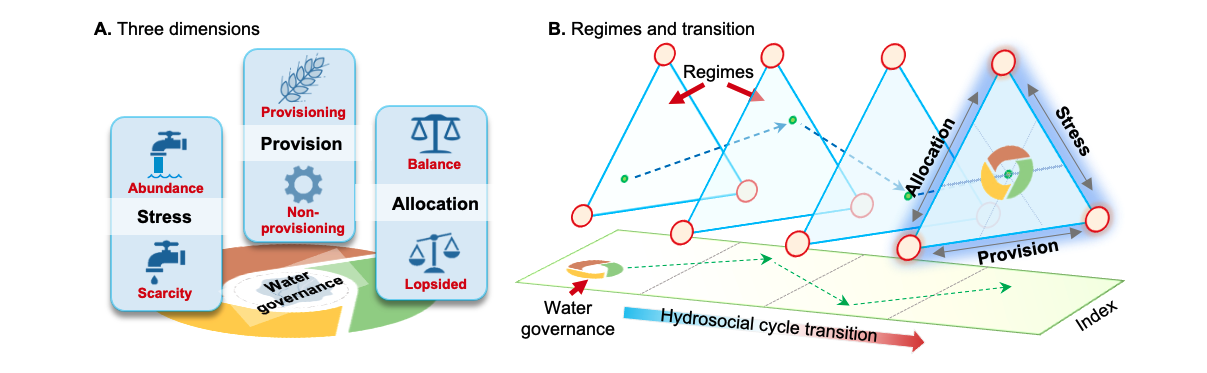
\includegraphics[width=0.9\textwidth]{main/framework.png}
	\caption{
		Identifying the water governance regimes in transitions of a hydrosocial cycle with an integrated water governance index (IWGI). Water stress (S), purposes of water services (P), and water allocation (A) are three aspects to be considered (\textbf{A.}). Along with hydrosocial-cycle transitions, a human-dominated regime influences these aspects of water governance. For example, the construction of reservoirs (1) aims to alleviate water stress; growth of energy and industry (2); water-lead intensive agriculture (3); conveyance system (4) controls water allocation.
		Therefore, the methodology is to combine three aspects' corresponding indicators, and then an abrupt change of the IWGI can indicate a regime shift in water governance (\textbf{B.}).
	}\label{fig:framework}
\end{figure*}


The Yellow River Basin (YRB), which contains the fifth-largest and most sediment-rich river in the world, needs integrated water governance because of geological and human history~\cite{mostern2021,best2019}.
Since the 1960s, governance practices such as reservoirs, levees, and conservation measures have contained the issues troubled by thousands of years of high sediment loads~\cite{wang2016e,song2020a}.
However, new challenges such as decreased streamflows and water depletions occurred in more recent times, leading to water use regulation and water transfer across basins -different focused water governance tactic~\cite{wang2019c}.
Today, it is still impossible to completely solve water stress, trade-offs between ecosystem services, or lopsided development in different regions in the YRB to the satisfaction of all actors~\cite{wohlfart2016a}.
Governance challenges induced by environmental, economic, social, and political factors have resulted in YRB being among the most intensively-governed large river basins worldwide~\cite{nickum2021}.
Identifying regime shifts in water governance within the YRB can thus provide crucial insights into rapidly-changing big river basins and how governance may respond to meeting challenges to their sustainability.

% 这里我们整合了三个方向,提出了描绘流域人水关系的指数
Here, we depict three aspects of water governance -stress, purpose and allocation with corresponding indicators (see methods) and thus develop an Integrated Water Governance Index (IWGI) by equally weighting them, to indicate results from water governance (see Figure~\ref{fig:framework}~B).
% 使用案例研究
Then, by applying the index to a typical rapid-changing big river basin (the YRB), we show how IWGI helps detect and describe complicated water governance regimes comprehensively but straightforwardly.
Following synthetic analyses of the changes in water demand, supply, economic outcomes, and institutions, we interpret the leading causes of the regime shifts.
% 最后总结出一般性框架
Finally, we propose a general regime transition schema that offers a practical guideline for a coordinated approach to exploring the challenges faced by big river basin governance.
